\documentclass{article}
\usepackage{pgfplots}
\pgfplotsset{compat=1.17}

\begin{document}

\begin{figure}[htbp]
    \centering
    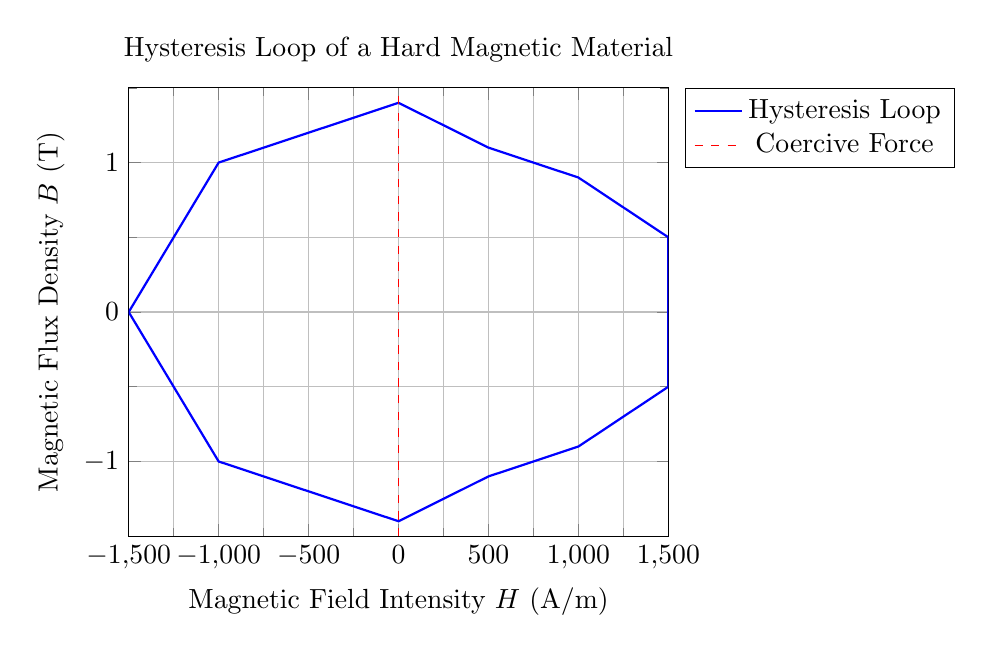
\begin{tikzpicture}
        \begin{axis}[
            xlabel={Magnetic Field Intensity $H$ (A/m)},
            ylabel={Magnetic Flux Density $B$ (T)},
            grid=both,
            minor tick num=1,
            legend pos=outer north east,
            title={Hysteresis Loop of a Hard Magnetic Material},
            xmin=-1500, xmax=1500,
            ymin=-1.5, ymax=1.5,
        ]
        % Define the hysteresis curve
        \addplot[thick, blue] plot coordinates {
            (-1500, 0) (-1000, 1.0) (-500, 1.2) (0, 1.4) (500, 1.1) (1000, 0.9) (1500, 0.5) 
            (1500, -0.5) (1000, -0.9) (500, -1.1) (0, -1.4) (-500, -1.2) (-1000, -1.0) (-1500, 0)
        };

        % Optional: add a dashed line for coercive force
        \addplot[dashed, red] coordinates {(0, -1.5) (0, 1.5)};

        \legend{Hysteresis Loop, Coercive Force}
        \end{axis}
    \end{tikzpicture}
    \caption{Hysteresis curve of a hard magnetic material showing the loop and coercive force.}
\end{figure}

\end{document}
